\documentclass[12pt,a4paper,titlepage,openany]{report}
\usepackage{zakljucna_FAMNIT_1_stopnja_MA_MEF_2016}
\usepackage{float}

% Glava dokumenta:

\fancyhf{}
\lhead[]{{\fontsize{9.3}{12}\selectfont
Priimek I. Naslov zaključne naloge.\\
\noindent Univerza na Primorskem, Fakulteta za matematiko, naravoslovje in informacijske tehnologije, leto}}
\chead[]{\fancyplain{}{}}
\rhead[]{\fancyplain{\thepage}
{\thepage}}
\cfoot[]{\fancyplain{}{}}
\lfoot[]{\fancyplain{}{}}
\rfoot[]{\fancyplain{}{}}
\normalsize

%%%%%%%%%%%%%%%%%%%%%%%%% ZAČETEK DOKUMENTA %%%%%%%%%%%%%%%%%%%%%%%%%%%%%%%%%%%%%%%%%%5

%%%%%%%%%%%%%%%%%%%%%%%%% Naslovna stran %%%%%%%%%%%%%%%%%%%%%%%%%


\begin{document}
\pagenumbering{Roman}
\pagestyle{empty}
\begin{center}
\noindent \large UNIVERZA NA PRIMORSKEM\\
\large FAKULTETA ZA MATEMATIKO, NARAVOSLOVJE IN\\
INFORMACIJSKE TEHNOLOGIJE


\normalsize
\vspace{6cm}
Zaključna naloga\\
\textbf{\large Nadzor porabe električne energije z namensko razvitim merilcem in  spletnim portalom}\\
\normalsize
(Control of electrical usage with dedicated measurer and  web portal)\\
\end{center}

\begin{flushleft}
\vspace{5cm}
\noindent Ime in priimek: Boštjan Vižintin
% v zgornjo vrstico dopišite ime in priimek študenta
\\
\noindent Študijski program: Računalništvo in informatika
% v zgornjo vrstico dopišite ime študijskega programa
\\
\noindent Mentor: doc. dr.  Peter Rogelj
% v zgornjo vrstico dopišite akademski naziv, ime in priimek mentorja

\end{flushleft}

\vspace{4cm}
\begin{center}
\large \textbf{Koper, Avgust 2017}
% dopišite mesec in leto oddaje zaključne naloge
\end{center}
\newpage

\pagestyle{fancy}
%%%%%%%%%%%%%%%%%%%%%%%%%%%%%%% Ključna dokumentacijska informacija (slo in ang) %%%%%%%%%%%

\section*{Ključna dokumentacijska informacija}

\medskip
\begin{center}
\fbox{\parbox{\linewidth}{
\vspace{0.2cm}
\noindent
Ime in PRIIMEK: Boštjan VIŽINTIN\vspace{0.5cm}\\
Naslov zaključne naloge: Nadzor porabe električne energije z namensko razvitim merilcem in  spletnim portalom\vspace{0.5cm}\\
Kraj: Koper\vspace{0.5cm}\\
Leto: 2017\vspace{0.5cm}\\
Število listov: 50 \hspace{2cm} Število slik: 20\hspace{2.6cm} Število tabel: 0\hspace{2cm}\vspace{0.5cm}\\
Število prilog: 1\hspace{1.9cm} Število strani prilog: 1\hspace{1cm} Število referenc: 17\vspace{0.5cm}\\
Mentor: doc. dr. Peter Rogelj\vspace{0.5cm}\\
Ključne besede: Nadzor porabe električne energije, Raspberry pi, spletni portal\vspace{0.5cm}\\
Math.~Subj.~Class.~(2010):\vspace{0.5cm}\\
{\bf Izvleček:}\\
Poraba električne energije v gospodinjstvih narašča in je v letu 2010 znašala približno 3.5 kWh na povprečno gospodinjstvo. Narašča tudi delež gospodinjstev opremljenih z dobrinami, ki za svoje delovanje potrebujejo elektriko. Ker gospodinjstva porabijo tretjino skupne električne energije, bi lahko z majhno spremembo porabe v posameznih gpospodinjstvih veliko vplivali na skupno porabo električne energije, vendar je to veliko enostavneje, če imamo natančen vpogled v porabo posameznih električnih naprav, ki si jih lasti gospodinjstvo. Glavna funkcija sistema bi torej bila nadzor porabe električne energije. V zaključni nalogi smo zato izdelali prototip za opravljanje meritev porabe električne energije na posamzenih uporabnikih, saj dandanes gospodinjstva nimajo natančnega pregleda v porabo električne energije. Sistem je zgrajen iz enostavnega merilca, ki je priključen na posamezne porabnike v gospodinjstvu, ta pa komunicira s centralno enoto. Uporabniki lahko nato preko spletnega portala preverijo porabo električne energije. Meritve se uporabniku prikažejo v obliki grafa in tabele, poleg porabe pa lahko uporabnik nastavi različna opozorila, ki bodo sprožena ob izbranih kriterijih.
\vspace{0.2cm}
}}
\end{center}

\newpage

\section*{Key words documentation}

\medskip

\begin{center}
\fbox{\parbox{\linewidth}{
\vspace{0.2cm}
\noindent
Name and SURNAME: Boštjan VIŽINTIN\vspace{0.5cm}\\
Title of final project paper: Control of electrical usage with dedicated measurer and  web portal\vspace{0.5cm}\\
Place: Koper\vspace{0.5cm}\\
Year: 2017\vspace{0.5cm}\\
Number of pages: 50\hspace{1.6cm} Number of figures: 20\hspace{2.2cm} Number of tables: 0\vspace{0.5cm}\\
Number of appendices: 1\hspace{0.6cm} Number of appendix pages: 1\hspace{0.8cm}Number of references: 20\vspace{0.5cm}\\
Mentor: Assist. Prof. Peter Rogelj, PhD\vspace{0.5cm}\\
Keywords: Control of electrical usage, Raspberry pi, web portal\vspace{0.5cm}\\
{\bf Abstract:}
Poraba električne energije v gospodinjstvih narašča in je v letu 2010 znašala približno 3.5 kWh na povprečno gospodinjstvo. Narašča tudi delež gospodinjstev opremljenih z dobrinami, ki za svoje delovanje potrebujejo elektriko. Ker gospodinjstva porabijo tretjino skupne električne energije, bi lahko z majhno spremembo porabe v posameznih gpospodinjstvih veliko vplivali na skupno porabo električne energije, vendar je to veliko enostavneje, če imamo natančen vpogled v porabo posameznih električnih naprav, ki si jih lasti gospodinjstvo. Glavna funkcija sistema bi torej bila nadzor porabe električne energije. V zaključni nalogi smo zato izdelali prototip za opravljanje meritev porabe električne energije na posamzenih uporabnikih, saj dandanes gospodinjstva nimajo natančnega pregleda v porabo električne energije. Sistem je zgrajen iz enostavnega merilca, ki je priključen na posamezne porabnike v gospodinjstvu, ta pa komunicira s centralno enoto. Uporabniki lahko nato preko spletnega portala preverijo porabo električne energije. Meritve se uporabniku prikažejo v obliki grafa in tabele, poleg porabe pa lahko uporabnik nastavi različna opozorila, ki bodo sprožena ob izbranih kriterijih.
\vspace{0.2cm}
}}
\end{center}




%%%%%%%%%%%%%%%%%%%%%%%%%%%%%%% Zahvala %%%%%%%%%%%%%%%%%%%%%%%%%%%%%%%%%%%%%

\newpage
\section*{Zahvala}

Zahvaljujem se mentorju, dr. Petru Roglju, za strokovno pomoč pri izdelavi zaključne naloge.

%%%%%%%%%%%%%%%%%%%%%%%%%%%%% Kazala %%%%%%%%%%%%%%%%%%%%%%%%%%%%%%
\newpage

% Dodamo kazala (po potrebi):
\tableofcontents
\addtocontents{toc}{\protect\thispagestyle{fancy}}
\newpage
\listoftables
\addtocontents{lot}{\protect\thispagestyle{fancy}}
\newpage
\listoffigures
\addtocontents{lof}{\protect\thispagestyle{fancy}}
\newpage
% ker priloge niso oštevilčene, tudi pikic do številk strani (ki jih ni) ne izpišemo
\renewcommand{\cftdot}{}
\listofappendices
\thispagestyle{fancy}
\newpage

\chapter*{Seznam kratic}
\thispagestyle{fancyplain}
\begin{longtable}{@{}p{1cm}@{}p{\dimexpr\textwidth-1cm\relax}@{}}
\nomenclature{$tj.$}{to je}
\nomenclature{$npr.$}{na primer}
\end{longtable}
\newpage

\normalsize

%%%%%%%%%%%%%%%%%%%%%%%%%%%%%%%%%% Poglavja: %%%%%%%%%%%%%%%%%%%%%%%%%%%%%%%%%%%%%

% Namig: Za večjo preglednost datoteke lahko vsebino vsakega poglavja shranite v poseben .tex dokument
% v isto mapo, kjer je shranjena osnovna .tex datoteka. Nato poglavja vstavite v dokument s klicem \include
% Primer: PrvoPoglavje.tex in DrugoPoglavje.tex vstavimo tako:
% \include{PrvoPoglavje}
% \include{DrugoPoglavje}

\chapter{Uvod}
\thispagestyle{fancy}
\pagenumbering{arabic}

\section{Definicija problema}
\thispagestyle{fancy}


Poraba električne energije v gospodinjstvih narašča in je v letu 2010 znašala približno 3.5 kWh na povprečno gospodinjstvo. Narašča tudi delež gospodinjstev opremljenih z dobrinami, ki za svoje delovanje potrebujejo elektriko. Na primer pomivalni stroj, stroj za sušenje perila, mobilni telefon, CD naprave, mikrovalovna pečica ter osebni računalnik. Kljub izboljšanju energetske učinkovitosti nekaterih naprav se poraba elektrike v povprečju ne znižuje, saj število naprav v gospodinjstvih narašča. Ker gospodinjstva porabijo tretjino skupne električne energije(http://shrinkthatfootprint.com/how-do-we-use-electricity), bi lahko z majhno spremembo porabe v posameznih gpospodinjstvih veliko vplivali na skupno porabo električne energije. Gospodinjstva redno prejemajo račune za količino porabljene električne energije vendar uporabniku skupna poraba električne energije ne koristi pri predstavi, kje v gospodijstvu bi lahko porabo omejil. Ideja je torej načrtovati in izdelati tak sistem, ki bi uporabnikom omogočal natančnejši nadzor porabe električne energije in s tem prikazal možnosti zmanjšanja električne energije.

\section{Predlog rešitve}
\thispagestyle{fancy}


Porabo električne energije v gospodinjstvih lahko zmanjšamo, vendar je to veliko enostavneje, če imamo natančen vpogled v porabo posameznih električnih naprav, ki si jih lasti gospodinjstvo. Glavna funkcija sistema bi torej bila nadzor porabe električne energije. Uporabniki bi lahko sami določili merilne točke in tako natačno izmerili porabo električne energije na posameznih merilnih mestih. Točna poraba bi bila nato prikazana za posamezna merilna mesta v obliki grafa. Poleg nadzora porabe, bi si lahko uporabniki določili različna opozorila. Sistem bi jih glede na opozorila opozarjal na preveliko uporabo oziroma na prekoračitev porabe električne energije in imel možnosti izklopa porabnikov v primeru sprožitve opozorila. Za lažjo predstavo o količini porabljene električne energije bi sistem omogočal tudi primerjavo porabe električne energije med seboj podobnimi gospodinjstvi.

\section{Težave}
\thispagestyle{fancy}

Ena od težav, ki nastopi pri merjenju porabe električne energije je montaža merilcev. Ker povprečno gospodinjstvo ne obvlada elektronike, bi morali biti merilci enostavni za montažo, sicer bi vsako montažo moral opraviti strokovnjak kar bi povečalo stroške in tako odvrnilo zanimanje s strani uporabnikov. Težave nastopijo tudi zaradi velike količine podatkov, ki jih merilne naprave konstantno pošiljajo na strežnik. 

\section{Študija izvedljivosti}
\thispagestyle{fancy}


\chapter{Analiza in definiranje zahtev}
\thispagestyle{fancy}

\begin{figure}[H]
\begin{center}
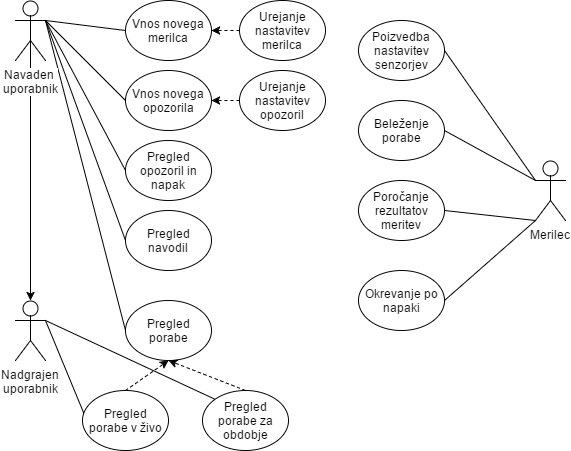
\includegraphics[width=1\textwidth, height=0.9\textheight,keepaspectratio]{Slike/UseCase.png}
\end{center}
\caption{Diagram primera uporabe.}\label{slika:UseCase}
\end{figure}

\newpage
Sistem za nadzor porabe električne energije bo na voljo vsem uporabnikom, ki bi želeli natančnejši pogled svoje porabe električne energije in tako potencialno zmanjšati porabo, kjer je to le možno. Sistem bo podpiral dve vrsti uporabnikov:
\begin{itemize}
\item Osnovne uporabnike
\item Nadgrajene uporabnike
\end{itemize}
Funkcije sistema bodo enake za vse uporabnike z razliko, da bodo imeli osnovni uporabniki nekaj omejitev pri nekaterih funkcijah kot na primer:
\begin{itemize}
\item Omejeno število meritev posameznega merilnega mesta na dan (manj natančna poraba)
\item Omejeno število dni hranjenja starih meritev
\item Omejeno število merilnih mest
\item Omejeno število nastavljivih opozoril
\end{itemize}


\section{Funkcijske zahteve}
\thispagestyle{fancy}


\subsection{Funkcijske zahteve merilca:}


\begin{itemize}
\item Poizvedba nastavitev senzorjev
\item Beleženje porabe
\item Poročanje rezultatov meritev
\item Okrevanje po napaki
\end{itemize}

\subsubsection{Poizvedba nastavitev senzorjev:}
Merilec bo imel zadnjo kopijo nastavitev shranjeno lokalno, zato da bo v primeru ko komunikacija med centralno enoto in merilcem ne bo vzpostavljena, lahko še vedno opravljal meritve. 
Ob vsakem zagonu, pred pričetkom opravljanja meritev, bo merilec poizkusil poslati zahtevo na centralno enoto, s svojim identifikacijskim nizom. V primeru da odgovora ne bo dobil, bo uporabil nastavitve, ki jih ima shranjene lokalno in si zabeležil napako(povezava s centralno enoto ni uspela). V primeru odgovora pa bo nastavitve posodobil in uporabil posodobljene nastavitve. 

\subsubsection{Opravljanje meritev:}
Glede na pridobljene nastavitve, bo merilec moral periodično opravljati meritve, za vsako merilno mesto posebej. 
\subsubsection{Poročanje rezultatov meritev:}
Po preteku periode, ki bo določena s strani posameznega uporabnika, bo merilec moral poslati meritve na centralno enoto. 
\subsubsection{Okrevanje po napaki:}
Vsaka napaka se bo beležila na merilcu  in se bo ob prvi možnosti posredovala na centralno enoto, kjer bo uporabnik imel pregled nad vsemi napakami. Po napaki pa mora merilec nadaljevati z opravljanjem meritev. Ena od napak je nedostopnost centralne enote. V tem primeru bo merilec uporabil lokalno kopijo nastavitev, vrednosti meritev pa bo shranjeval lokalno, dokler povezava s centralno enoto ne bo vzpostavljena. 

Drugi problem je izpad elektrike. V tem primeru se bo merilec izklopil, ob vzpostavitvi elektrike pa se mora merilec sam zagnati, ter pognati program za opravljanje meritev.


\begin{figure}[H]
\begin{center}
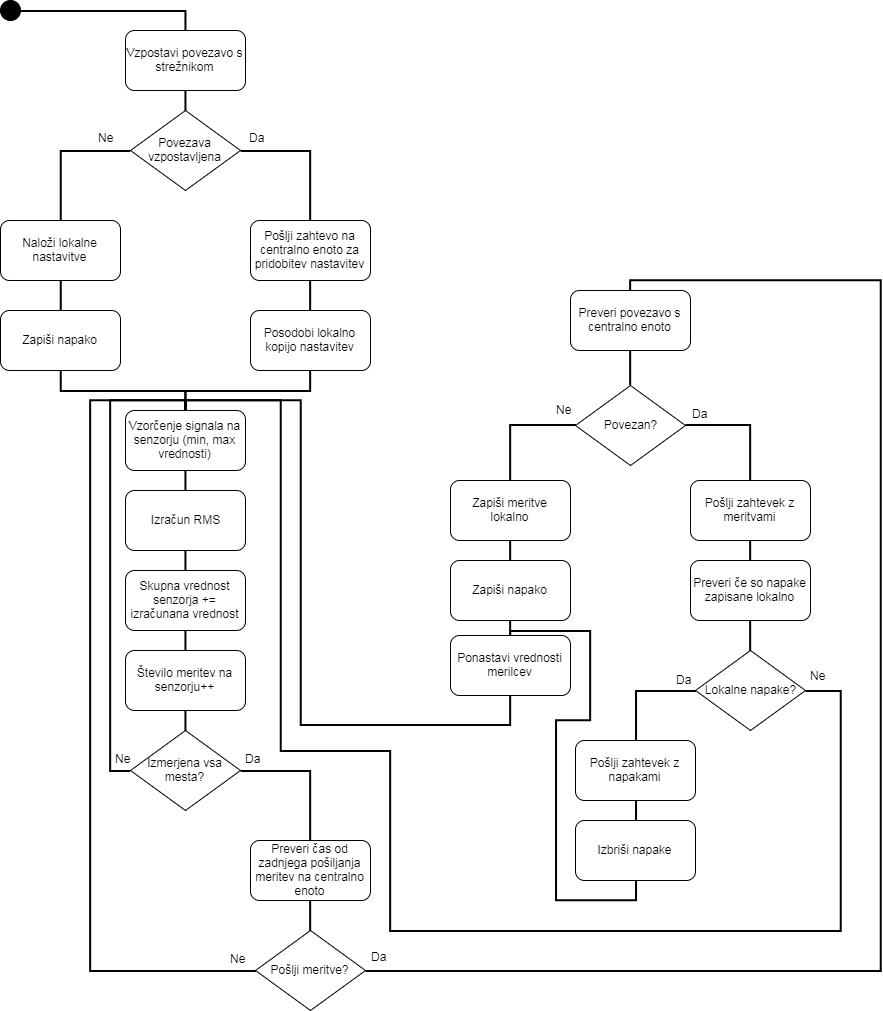
\includegraphics[width=1\linewidth]{Slike/ActivityMerilec.png}
\end{center}
\caption{Diagram aktivnosti za merilec.}\label{slika:ActivityMerilec}
\end{figure}

\newpage
\subsection{Funkcijske zahteve aplikacije:}



\begin{itemize}
\item Vnos novega merilca
\item Urejanje in konfiguracija vnešenih merilcev
\item Pregled porabe električne energije po merilnih mestih z možnostjo različnih filtrov
\item Pogled porabe posameznega senzorja "v živo"
\item Dodajanje novih opozoril
\item Urejanje že vnesenih opozoril
\item Pregled napak in opozoril sistema
\item Nadgradnja uporabnika v plačljivega uporabnika
\item Pregled navodil za uporabo
\end{itemize}

\subsubsection{Vnos novega merilca:}
Na portalu bomo po pritisku gumba za vnos novega merilca preusmerjeni na formo za vnos novih merilcev. Vnos merilca mora uporabniku preko enostavnih vnosnih polj omogočati vnos novega merilca. Za vno novega merilca bo potreben vnos imena, identifikacijskega niza in števila priključenih senzorjev. Po vnosu merilca, se bo ta prikazal v meniju, kjer bo uporabnika po pritisku na merilec, preusmerilo na stran za urejanje nastavitev merilca ter senzorjev, ki so na njega priključeni.

\begin{figure}[H]
\begin{center}
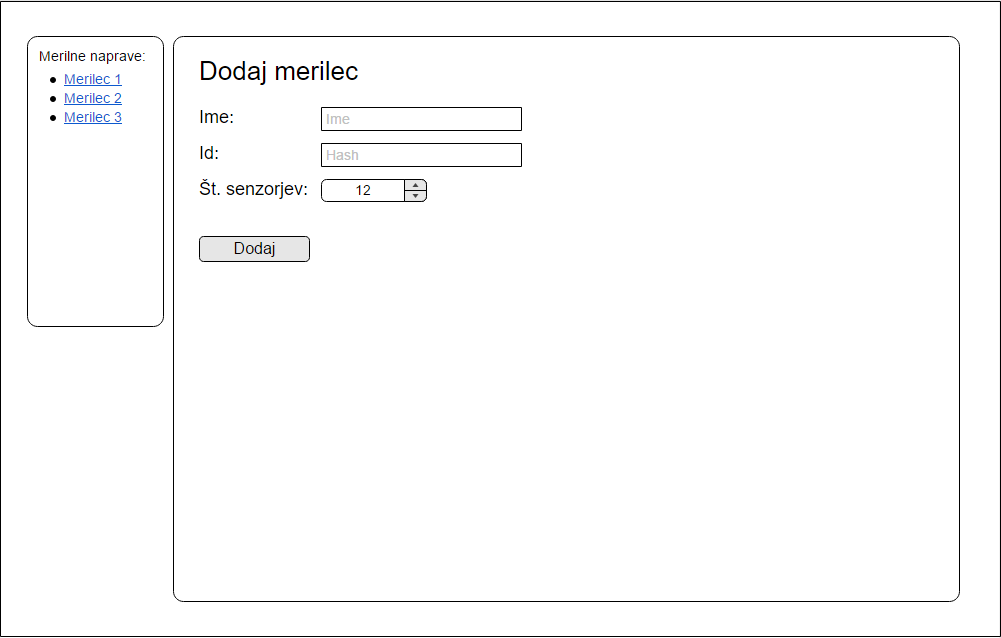
\includegraphics[width=1\linewidth]{Slike/VnosNovegaMerilca.png}
\end{center}
\caption{Vnos novega merilca.}\label{slika:VnosNovegaMerilca}
\end{figure}

\subsubsection{Urejanje in konfiguracija vnešenih merilcev:}
Po pritisku na ime merilca bo uporabnika preusmerilo na stran za urejanje in konfiguracijo vnešenih merilcev. Tukaj bo uporabnik lahko nastavil vse možne nastavitve, ki so povezane z delovanjem merilcev.

\begin{itemize}
\item ime merilca
\begin{flushleft}
Urejanje imena merilca, če si uporabnik želi spremeniti ime, ki ga je izbral ob vnosu merilca.
\end{flushleft}
\item število priključenih senzorjev
\begin{flushleft}
Urejanje števila priključenih senzorjev, če je uporabnik dodal/odstranil senzorje iz merilca.
\end{flushleft}
\item periodo sporočanja meritev
\begin{flushleft}
Izbira časovnega intervala, ki pove na koliko časa merilec posreduje meritve na centralno enoto.
\end{flushleft}
\item razporeditev priključenih senzorjev
\begin{flushleft}
Izbira vhoda na katerega je priključen senzor.
\end{flushleft}
\item ime posameznega merilnega mesta
\begin{flushleft}
Vnos imena posameznega merilnega mesta oziroma senzorja, za lažjo prepoznavo merilnih mest pri prikazu porabe.
\end{flushleft}
\item tip senzorja
\begin{flushleft}
Izbira tipa senzorja npr. 5A, 20A, 30A.
\end{flushleft}
\item trajanje vzorčenja
\begin{flushleft}
Vnos trajanja vzorčenja signala posameznega senzorja.
\end{flushleft}
\end{itemize}


\begin{figure}[H]
\begin{center}
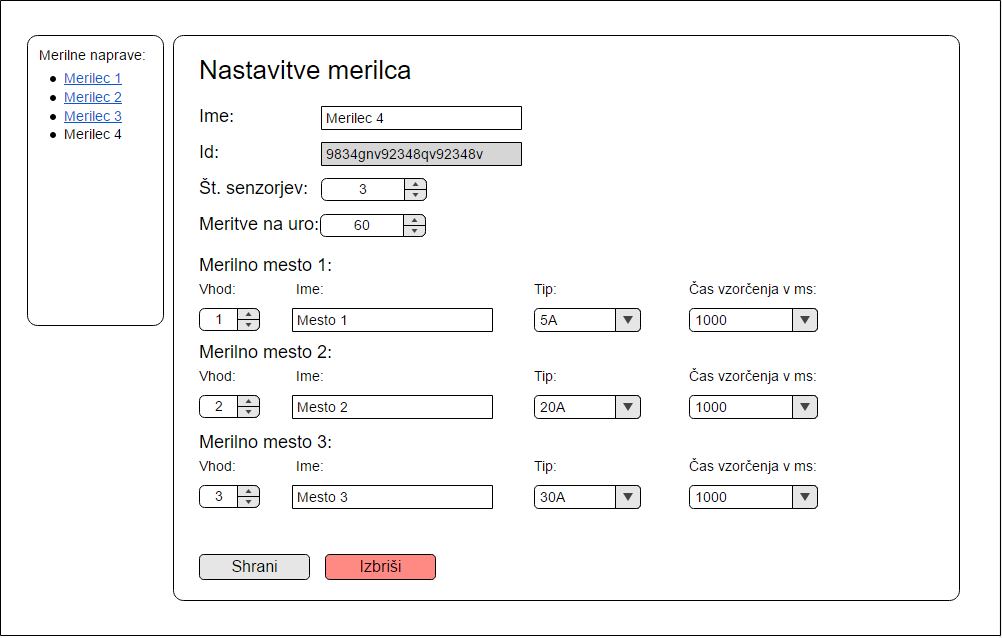
\includegraphics[width=1\linewidth]{Slike/UrejanjeMerilca.png}
\end{center}
\caption{Nastavitve merilca.}\label{slika:UrejanjeMerilca}
\end{figure}

\subsubsection{Pregled porabe električne energije po merilnih mestih z možnostjo različnih filtrov:}

\begin{figure}[H]
\begin{center}
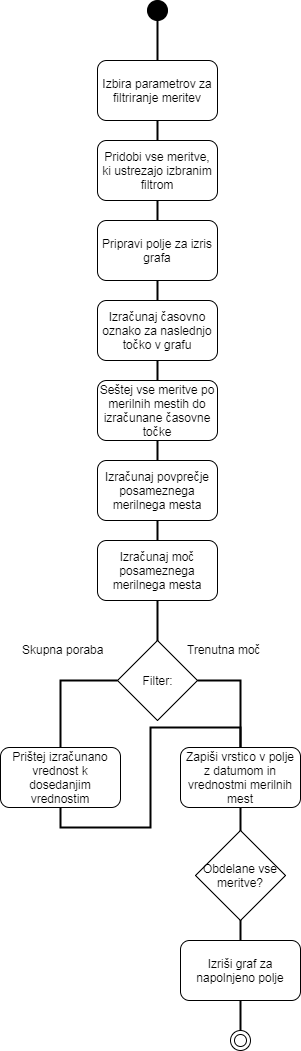
\includegraphics[width=1\textwidth, height=0.9\textheight,keepaspectratio]{Slike/ActivityPoraba.png}
\end{center}
\caption{Diagram aktivnosti za pregled porabe.}\label{slika:ActivityPoraba}
\end{figure}


Na portalu bomo po pritisku gumba za pregled meritev preusmerjeni na formo za izbiro parametrov pri pregledu porabe. Uporabnik bo lahko izbiral med vsemi svojimi merilci, za vsak merilec pa bo označil samo tista merilna mesta oziroma senzorje, za katere bo želel videti porabo. Z vnosom datumov in ur bo omejil prikaz porabe na točno določeno obdobje, z izbiro intervala pa bo izbral razdaljo med točkami prikaza porabe na grafu (npr. po minutah, urah, ...). Možna bo tudi izbira prikaza porabe po trenutni moči ali pa skupni porabi.

\begin{figure}[H]
\begin{center}
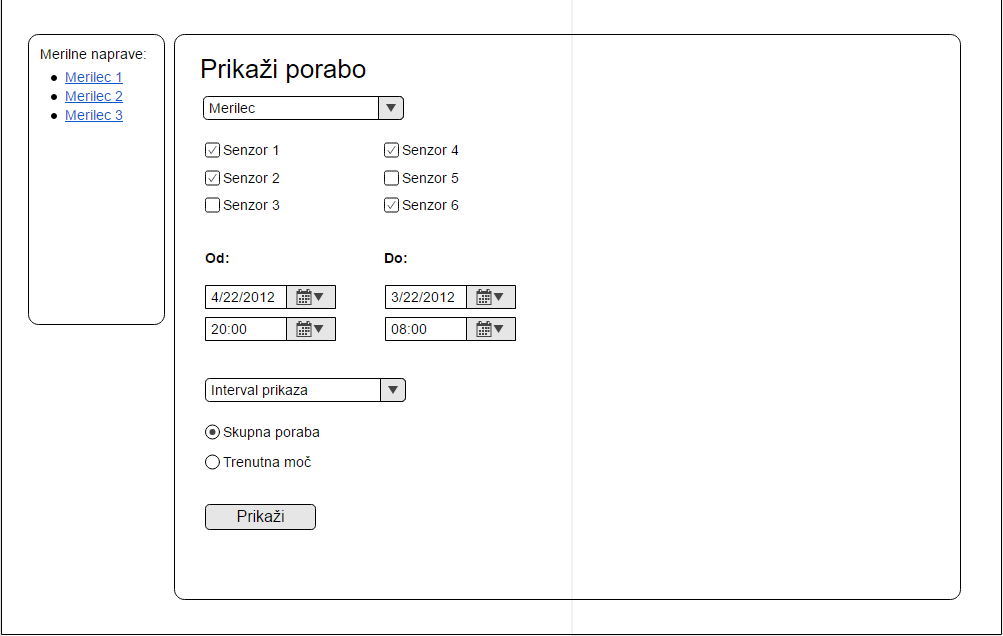
\includegraphics[width=1\linewidth]{Slike/IzbiraPregledaPorabe.png}
\end{center}
\caption{Filter pregleda porabe.}\label{slika:IzbiraPregledaPorabe}
\end{figure}

\subsubsection{Pregled porabe posameznega senzorja "v živo":}
Po vnosu vseh želenih parametrov za prikaz porabe, bo uporabnik preusmerjen na stran, kjer bo graf, ki bo prikazoval porabo za vse izbrane senzorje, glede na izbrane parametre. Možen bo izklop prikaza porabe za posamezna merilna mesta, zato da bojo ostala merilna mesta lažje vidna. S pritiskom na ime merilnega mesta pa bo uporabnika preusmerilo na graf, kjer bo prikazana poraba samo izbranega senzorja, ta pa se bo osveževala vakokrat ko bo centralna enota prejela novo meritev za izrani senzor.

\begin{figure}[H]
\begin{center}
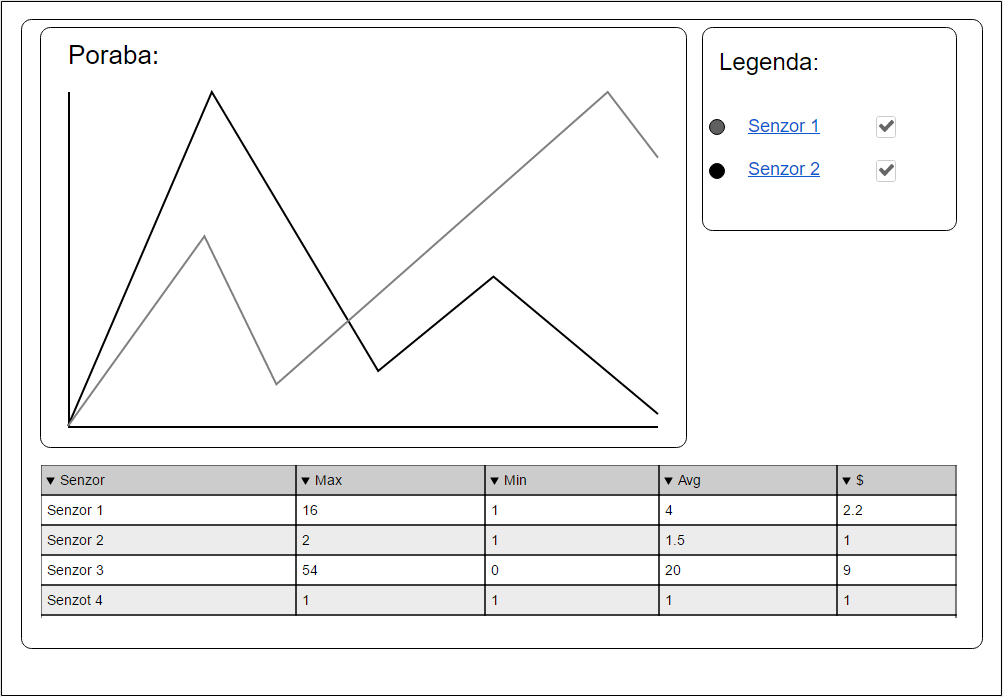
\includegraphics[width=1\linewidth]{Slike/PregledPorabe.png}
\end{center}
\caption{Pregled porabe.}\label{slika:PregledPorabe}
\end{figure}

\subsubsection{Dodajanje novih opozoril:}
Na portalu bomo po pritisku gumba za vnos opozoril preusmerjeni na formo za vnos novih opozoril. Uporabnik bo vnesel ime opozorila, izbral merilec in merilno mesto, nastavil vrednost, pri kateri želi da se opozorilo sproži ter izbral obdobje, med katerim bo opozorilo veljavno.


\begin{figure}[H]
\begin{center}
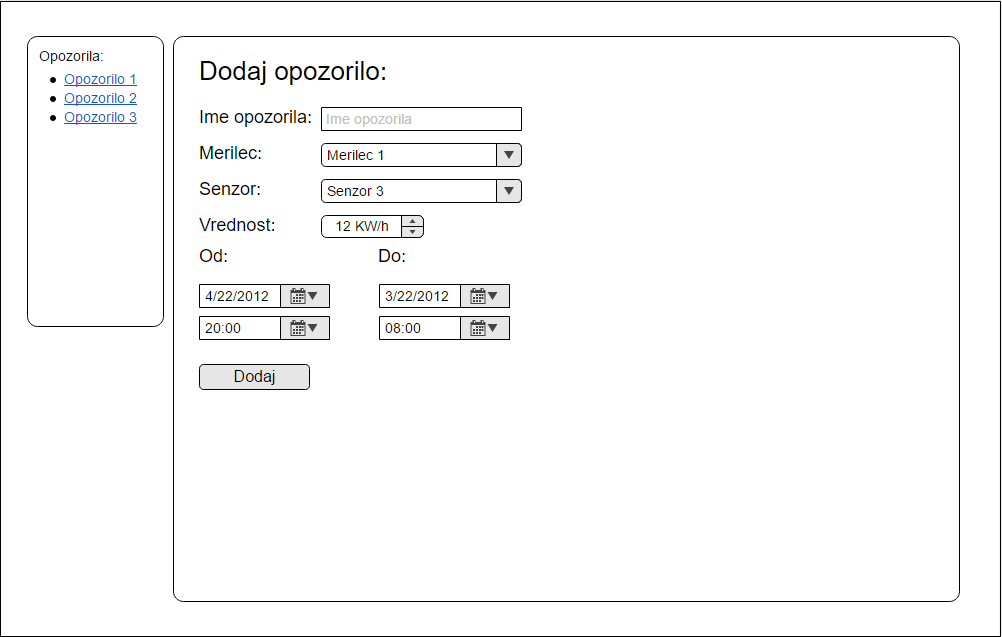
\includegraphics[width=1\linewidth]{Slike/DodajOpozorilo.png}
\end{center}
\caption{Dodajanje novega opozorila.}\label{slika:DodajOpozorilo}
\end{figure}

\subsubsection{Urejanje vnesenih opozoril:}
Po izbiri že vnesenega opozorila bo uporabnika preusmerilo na formo kjer bo lahko uporabnik uredil podatke ki jih je vnašal pri vnosu tega opozorila.

\begin{figure}[H]
\begin{center}
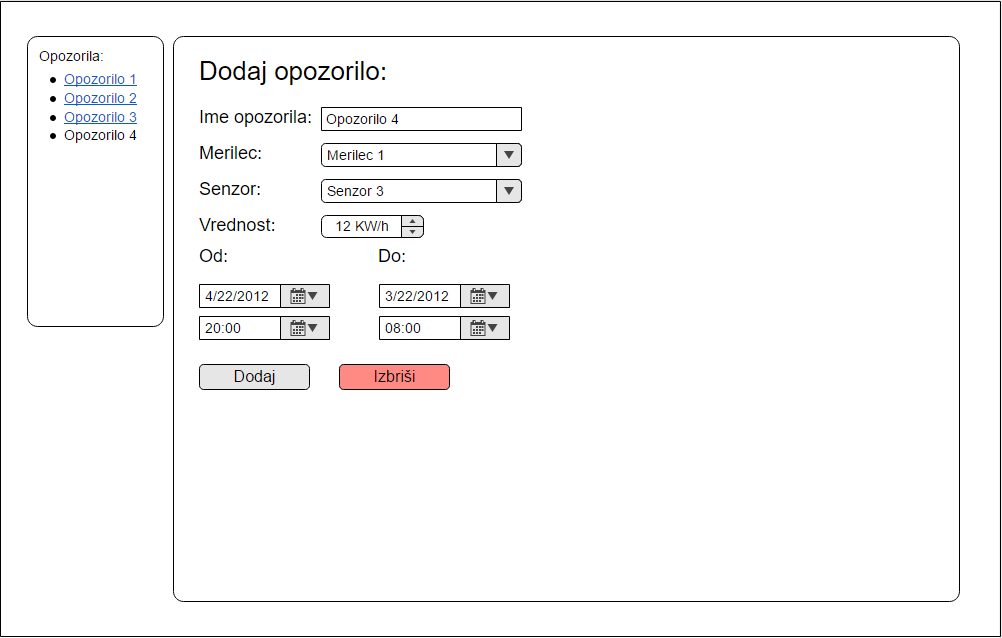
\includegraphics[width=1\linewidth]{Slike/UrediOpozorilo.png}
\end{center}
\caption{Urejanje opozorila.}\label{slika:UrediOpozorilo}
\end{figure}

\subsubsection{Pregled napak in opozoril sistema:}
Na portalu bomo po pritisku gumba za pregled opozoril preusmerjeni na stran, kjer se bojo prikazovale napake sistema/merilcev in opozorila uporabnika. 

\begin{figure}[H]
\begin{center}
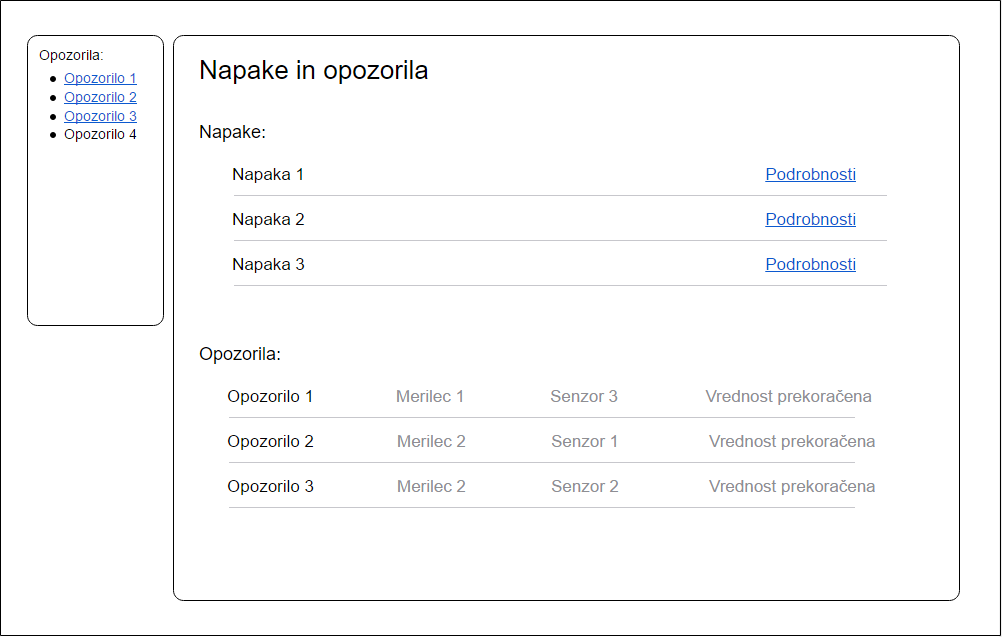
\includegraphics[width=1\linewidth]{Slike/PregledOpozorilInNapak.png}
\end{center}
\caption{Pregled opozoril in napak.}\label{slika:PregledOpozorilInNapak}
\end{figure}


\subsubsection{Nadgradnja uporabnika v nadgrajenega uporabnika:}

????????????????????

\subsubsection{Pregled navodil za uporabo:}

Na portalu bomo po pritisku gumba za navodila preusmerjeni na stran kjer bojo zapisana navodila za priklop senzorja, razne informacije in opisi možnih nastavitev senzorjev ter opis uporabe spletnega portala.

\section{Nefunkcijske zahteve}
\thispagestyle{fancy}


\subsection{Nefunkcijske zahteve merilca:}

\begin{itemize}
\item Varnost
\item Cena
\item Prenosljivost
\end{itemize}

\subsubsection{Varnost:}

Pri uporabi merilca moramo biti pozorni na dve stvar, ki predstavljajo problem z varnostjo. Prvi problem predstavlja upravljanje z visoko napetostjo, ki je lahko usodna. Drugi problem je varovanje podatkov o uporabniku in meritvah.

\begin{itemize}
\item Visoka napetost

Na največji problem pri varnosti naletimo pri priklopu merilca na posamezne porabnike. Ker uporabljamo senzor, ki za svoje delovanje zahteva direkten priklop na porabnike, lahko pri priklopu pridemo v neposreden stik z električno napetostjo, kar je lahko usodno. Problem je torej da mora uporabnik prerezato žico, odstranit izolacijo in porabnik priključiti v senzor. Problem lahko delno rešimo z uporabo drugačnih senzorjev, na primer senzorji ki za svoje delovanje ne potrebujejo direktnega priklopa. En primer je ZGORAJ OMENJENI SENZOR, ki za svoje delovanje potrebuje samo žico porabnika, ki je speljana skozi tuljavico. Nevarnost za neposreden stik bi s takim senzorjem nekoliko zmnjšali, vendar še vedno obstaja nevarnost, zato bi uporabnikom brez znanja na tem področju, merilno napravo moral namestiti strokovnjak. Za priklope na enostavnejše porabnike pa bi izdelali senzorje ki bi bili vgrajeni v "adapter" za električne vtičnice ali celo razdelilce.

\item Varovanje podatkov

Merilna naprava konstantno pošilja veliko količino meritev na centralno enoto. Pozorni moramo biti na možnost, da bi lahko ljudje s slabimi nameni simulirali merilce uporabnikov in tako pošiljali napačne podatke na centralno enoto, kar bi se opazilo kot napačno porabo. Problem lahko rešimo z uporabo varnega protokola HTTPS pri pošiljanju meritev iz merilca na centralno enoto.

\end{itemize}


\subsubsection{Cena:}

Cena merilca mora biti ugodna, saj je glavna ideja sistema znižanje stroškov porabe električne energije, torej bi visoka cena odvrnila uporabnike, saj bi samo nakup sistema za opravljanje meritev povečal stroške. Merilec mora biti tudi do velike mere prilagodljiv na uporabnikove zahteve, tako bo lahko uporabnik, ki želi opravljati meritve le na malem številu porabnikov, kupil merilec z manj senzorji, kar bi pomenilo manjši strošek.

\subsubsection{Prenosljivost:}

Velikost merilca je pomembna saj mora biti merilec prenosljiv, zato da ga lahko uporabnik uporablja na željenih mestih. Velikost merilca igra vlogo tudi zaradi možnosti montaže na mesta, ki niso bila izdelana z namenom proklopa dodatne opreme npr. škatla z varovalkami. 

\subsection{Nefunkcijshe zahteve aplikacije:}


\subsubsection{Registracija/prijava uporabnika v sistem:}

Sistem mora podpirati registracijo novih uporabnikov in prijavo že registriranih uporabnikov, zaradi varovanja podatkov in pa tudi zaradi shrambe nastavitev merilcev, saj mora sistem vedeti katere nastavitve spadajo k določenemu senzorju.



\chapter{Načrtovanje sistema}
\thispagestyle{fancy}

\begin{figure}[H]
\begin{center}
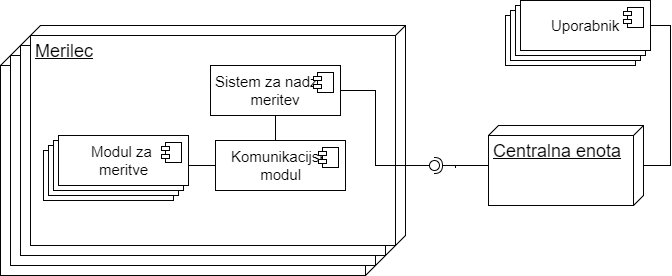
\includegraphics[width=1\linewidth]{Slike/NacrtSistema.png}
\end{center}
\caption{Načrt sistema.}\label{slika:NacrtSistema}
\end{figure}

\section{Načrtovanje merilca}
\thispagestyle{fancy}

\subsection{Metode merjenja toka}
Zazanavanje toka je uporabljeno za izvajanje dveh poglavitih funkcij. Meri se količina toka, ki teče skozi porabnik, kar lahko uporabimo za nadzor porabe in meri se previsok tok oziroma napake. Če tok preseže varne meje, programska ali strojna oprema lahko ustrezno reagira in izklopi delovanje naprave. Za opravljanje meritev toka poznamo veliko načinov:

\begin{itemize}
\item Resistive (direktno merjenje)

\begin{itemize}
\item Current sense resistors
\end{itemize}

 \item Magnetno (indirektno merjenje)

\begin{itemize}
\item Current transformer
\item Rogowski coil
\item Hall effect device
\end{itemize}

\item Transistor (direktno merjenje)

\begin{itemize}
\item RDS(ON)
\item Ratio-metric
\end{itemize}

\end{itemize}

http://www.vishay.com/docs/30304/currentmeasurement.pdf

Vsaka od metod merjenja ima prednosti in slabosti, ki so ključne ko izbiramo metodo in vrsto zenzorja, ki ga bomo uporabili
v naši aplikaciji. Metode merjenja so razdeljene v dve glavne kategorije: direktno merjenje in indirektno merjenje.
Direktno merjenje pomeni, da je senzor oziroma naprava za merjenje toka priključena direkno na izvor pod napetostjo, 
indirektno merjenje pa pomeni, da je senzor oziroma naprava za merjenje toka nekako ločena od izvora napetosti, 
kar je lahko ključno za varnost aplikacije.

\subsubsection{Resistive:}
\subsubsection{Current Sense Resistor}
Metoda merjenja toka z upornostjo je enostavna in linearna metoda. Upor na katerm se meri tok, namestimo vzporedno z porabnikom na katerem želimo izmeriti tok.
Majhen tok poskrbi, da se majhna količina moči pretvori v toploto. Pretvorba moči v toploto poskrbi za napetostni signal. Poleg enostavnosti merjenja, dobrih karakteristik, linearnosti, 
konstantnim temperaturnim koeficientom upornosti, je metoda merjenja toka z uporanostjo zelo poceni. S to metodo se zavarujemo tudi proti kratkim stikom in premočnim tokom.

\subsubsection{Magnetic:}
\subsubsection{Current Transformer}
Tokovni transformator ima tri ključne prednosti: izolacijo od porabnika, neizgubno tokovno merjenje in velik napetostni signal, ki je neobčutljiv na motnje. Z uporabo te metode lahko merimo izmenične, prehodne ali modulirane enosmerne tokove. Omenjeni tokovi spreminjajo magnetno polje ki se prenese v sekundarno navitje transformatorja. Skalo merjene napetosti na sekundarnem navitju lahko spreminjamo s spremembo razmerja ovojev na primarnem in sekundarnem navitju. Metoda se smatra za neizgubno, saj tok teče po bakrenem navitju z zelo majhno izgubo zaradi upornosti, vendar pa vseeno izgubimonekaj moči zaradi obremenilnega upora, izguba jedra in primarnega in sekundarnega enosmernega upora.

\subsubsection{Rogowski Coil}
Metoda z uporabo Rogowske tuljave je podobna metodi z uporabo tokovnega transformatorja v tem, da je napetost inducirana na sekundarnem navitju, ki je proporcionalna toku, ki teče skozi izolirani prevodnik. Razlikujeta se v tem, da jedra pri Rogovski tuljavi ni v nasprotju z tokovnim transformatorjem, kjer je jedro iz železa. Rogowka tuljava ima zaradi tega nižjo induktanco, zaradi česar dosežemo hitrejši odziv signaloc in zelo linearen napetostni signal. Zaradi svojega dizajna je pogosto uporabljea kot začasna metoda za merjenje toka na instrumentih za merjenje toka. Smatramo jo za nižje cenovno alternativo metodi merjenja toka s tokovnim transformatorjem.

\subsubsection{Hall Effect}
Ko postavimo porabnik skozi katerega teče tok, v magnetno polje, se pojavi razlika potencialov pravokotno na magnetno polje in na smer v katerga teče tok. Ta potencial je sorazmeren moči toka, ki teče skozi porabnik. Napetost ki jo lahko izmerimo zaradi razlike potencialov imenujemo Hallova napetost. Z napravami, ki uporabljajo Hallov efekt lahko merimo velike toke z majhno izgubo moči. Poleg dobrih lastnosti pa imamo tudi slabe lastnosti, kot so ne linearne meritve pri razlikah temperature (problem rešimo z kompenzacijo), omejena pasovna širina, majhno območje meritev ( problem rešimo z velikim napetostnim zamikom, kar predstavi nova odstopanja), občutljivost na zunanja magnetna polja in visoko ceno.

\subsubsection{Transistor:}
\subsubsection{RDS(ON) - Drain-to-Source On-Resistance}


Transistors are considered a “lossless” overcurrent detection method since they are standard control components to the circuit
design and no further resistance or power dissipating devices are required to provide a control signal. Transistor datasheets
provide the on-resistance for the drain-to-source (RDS(ON)) with a typical resistance in the m range for power MOSFETs. This
resistance consists of several components that begin with the leads (Fig. 6) connecting to the semiconductor die through the
resistance that makes up the numerous channel characteristics. Based on this information, the current passing through the
MOSFET can be determined by ILoad = VRDS(ON) / RDS(ON).
Each constituent of the RDS(ON) contributes to measurement errors that are due to minor variations in the resistances of the
interface regions and TCR effects. The TCR effects can be partially compensated by measuring temperature and correcting the
measured voltage with anticipated changes in resistance due to temperature. Often times the TCR for MOSFETs can be as large
as 4000 ppm, which is equivalent to a 40  change in resistance for a 100  rise. Generally, this measurement method
provides a signal with approximately 10  to 20  accuracy. Depending on the accuracy requirements, this may be an
acceptable range for providing overcurrent protection.

\subsubsection{Ratio Metric - Current Sense MOSFETs}
The MOSFET consists of thousands of parallel transistor cells that reduce the on-resistance. The current sensing MOSFET uses
a small portion of the parallel cells and connects to the common gate and drain, but a separate source (Fig. 7). This creates a
second isolated transistor; a “sense” transistor. When the transistor is turned on, the current through the sense transistor will
be a ratio comparable to the main current through the other cells.
Depending on the transistor product, the accuracy tolerance range can vary from as low as 5  to as wide as 15  or 20 .
This is generally not suitable for current control applications that typically require 1  measurement accuracy, but is intended
for overcurrent and short circuit protection.

\subsection{Senzor ACS712}
Senzor ki smo ga izbrali je ACS712.


\begin{figure}[H]
\begin{center}
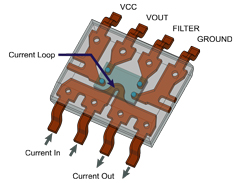
\includegraphics[width=0.5\linewidth]{Slike/ACS712.jpg}
\end{center}
\caption{ACS712.}\label{slika:ACS712}
\end{figure}

Senzor obstaja v treh različicah in sicer:

\begin{itemize}
\item ACS712ELCTR-05B-T
\item ACS712ELCTR-20A-T
\item ACS712ELCTR-30A-T
\end{itemize}

Razlikujejo se v občutljivosti oziroma koliko voltov razlike dobimo na izhodu za vsak izmerjen amper na vhodu, kar vpliva na to, kakšen je maksimalen tok ki ga lahko izmerimo. Kot je iz imen senzorjev razvidno so senzorji primerni za toke do 5A(185mV/a), 20A(100mV/A) in 30A(66mV/A) kot si sledijo.


SLIKA MOJIH SENZORJEV

Senzorji, ki smo jih uporabili za izdelavo prototipa smo kupili v obliki modulov(zgoraj omenjen senzor, z vso potrebno periferijo za takojšnji priklop in uporabo). Senzorji imajo sicer sponko za priklop porabnika, vendar je merjenje vseeno indirektno, saj je senzor galvansko ločen. Zaradi potrebe po reaznju žice porabnika, za priklop senzorja, ta oblika senzorja ni najbolj optimalna za končni izdelek, za izdelavo prototipa pa bo zadostovala. Na spodnji sliki je senzor, ki je varnajši za priklop.

SLIKA PRIMERNEJŠEGA SENZORJA.

\subsection{Analogno digitalni pretvornik MCP3008}
MCP3008 je nizkocenovni 8 kanalni 10 bitni analogno digitalni pretvornik. Natančnost tega čipa je podobna čipu uporabljenem na Arduino UNO. V primeru da bi kasneje želeli natančnejše meritve bi morali ta čip zamenjati za natančnejši čip na primer: ADS1015(12 bit) ali še natančnejši ADS1115(16 bit). Komunikacija med Raspberry Pi in MCP3008 poteka po SPI protokolu.

\subsection{SPI}
SPI(ang. Serial Peripheral Interface bus) je standard za sinhrono serijsko podatkovno povezavo, ki je uporabljena za kratke povezave. Najpogosteje je uporabljena v vgrajenih sistemih. Standard je bil razvit leta 1980, razvila pa ga je Motorola. Kmalu za tem je postal "de facto" standard. Tipično uporabo SPI vodila lahko zasledimo pri Secure Digital karticah (SD) in pri LCD zaslonih. Naprave ki uporabljajo SPI protokol, komunicirajo med seboj v dvosmernem načinu(full duplex), s principom nadrejenega/podrejenega(master/slave), z enim nadrejenim(master) in možnostjo več podrejenih(slave), katere nadrejeni izbira preko SS vodila. Včasih SPI-ju rečemo kar štiri žično serijsko vodilo, ker za svojo delovanje uporablja štiri žice.

\begin{itemize}
\item MOSI: MOSI priklop je uporabljen za prenos podatkov iz SPI modula, ko je nastavljen kot nadrejeni in za sprejem podatkov ko je nastavljen kot podrejeni.
\item MISO: MISO priklop je uporabljen za prenos podatkov iz SPI modula, ko je nastavljen kot podrejeni in za sprejem podatkov ko je nastavljenkot nadrejeni.
\item SS: This pin is used to output the select signal from the SPI module to another peripheral with which a data transfer is to take place when its configured as a Masterand its used as an input to receive the slave select signal when the SPI is configured as Slave.
\item SCK: SCK priklop je uporabljen za izhod urinega signala, kateri določa takt prenosa podatkov med nadrejenim/podrejenim.
\end{itemize}

\subsection{Arduino ali Raspberry Pi}
Arduino je odprtokodna elektronska platforma zgrajena z hardwerom in softwerom ki je lahek za uporabo. Nastal je na inštitutu Ivrea Interaction Design, kot orodje za hitro izdelavo prototipov, namenjen pa je bil za študente brez predhodnega znanja elektrotehnike in programiranja. Kmalu za tem je postal zelo priljubljen in posledično se je začel razvijat. Zmore od enostavnih projektov kot so aktivacija motorja, prižiganje luči, branje senzorja pa do 3D printanja in uporabo v vgrajenih sistemih, uporabljajo ga pa tako začetniki kot tudi profesionalci. Na voljo je več verzij Arduinota, ki pa se razlikujejo predvsem v verziji mikrokontrolerja od katerega je tudi odvisno številov digitalnih in analognih vhodov in izhodov ter ceni, ki znaša od od 20 do 80 evrov. Ker je platforma kot že omenjeno odprtokodna pa seveda lahko dobimo Arduino ploščice pod drugim imenom, z enako funkcionalnostjo za veliko ceneje. Zaradi cene, razširjene uporabe platforme in obsežne dokumentacije, ki je na voljo na spletu, je bil Arduino kandidat za izdelavo naprave za diplomsko nalogo. Kasneje se je izkazalo, da je Raspberry pi nekoliko bolj     primeren.

Kot že omenjeni Arduino je bil Raspberry Pi namenjen promoviranju in učenju osnov računalništva. Vsi modeli Raspberry Pi vsebujejo Broadcom-ov Soc(System on a chip), kateri je zgrajen iz ARM-ovega procesorja (CPU) in grafičnega procesorja GPU. Ure procesorjev so med 700MHz in 1.2GHz, pomnilnik pa varira med 256MB in 1GB RAM. Za shrambo operacijskega sistema je uporabljena Secure Digital (SD) kartica različnih velikosti. Večina ploščic ima med 1 in 4 USB vhodov, HDMI in composit video izhod, 3.5mm audio jack. Nižje razredni vhodi/izhodi so na voljo preko številnih GPIO pinov, ki podpirajo protokole kot na primer I2C. Nekatere ploščice imajo tudi Ethernet port in WIFI ter bluetooth. Deluje na operacijskem sistemu raspbian, ki je Debianova različica linuxove distribucije.

Za razvoj merilnika za naše potrebe, razvojna ploščica Arduino zadostuje vsem zahtevam, zato je bila prva verzija merilnega instrumenta izdelana z Arduino ploščico verzijo Arduino UNO. Arduino je s pomočjo senzorjev uspešno opravljal meritve, vendar je bil nestabilen in sicer pri večkratnem zaporednem pošiljanju requestov na strežnik  je "zmrznil". Ker težave nismo uspeli odpraviti smo zato Arduino zamenjali z Raspberry Pi. Raspberry Pi se je izkazal enostavnejši za uporabo ( naprednejši jezik???? ), vendar smo pri zamenjavi naleteli na novo težavo in sicer Raspberry Pi nima analognih vhodov ( Arduino ima vgrajene analogno digitalne pretvornike na ploščici). Problem smo rešili z uporabo analogno/digitalnega pretvornika MCP3008.



\subsection{RMS - Root mean square}

Za določeno število vrednosti n diskretne porazdelitve xi, ..., xn, root mean square (krajše RMS, včasih imenovan tudi
quadratic mean), je kvadratni koren povprečja vrednosti vseh xi na kvadrat.

FORMULA

Zgornji izračun lahko nekoliko poenostavimo, če vemo da je signal katerega želimo izračunati RMS vrednost, sinusoiden.
Periodična sinusoidna napetost je konstanten in je definiran kot V(t) = Vm*cos(wt) s periodo T. Tako lahko izračunamon RMS
vrednost sinusoidne napetosti V(t) kot

FORMULA

http://www.electronics-tutorials.ws/accircuits/rms-voltage.html
http://mathworld.wolfram.com/Root-Mean-Square.html


\subsection{Hitrost vzorčenja:}
Eden od problemov pri merjenu izmeničnega toka je ta, da senzor meri samo trenutno vrednost. Ker je merjeni signal(izmenični) sinusne oblike, to pomeni da bi lahko za enak porabnik, izmeril več različnih vrednosti, odvisno od časa opravljene meritve.

SLIKA SINUSA Z OZNAČENIMI MERITVAMI KI KAŽEJO DRUGAČNE VREDNOSTI.

Za točno meritev moremo torej s pomočjo meritev izračunati RMS(root mean square) vrednost. Za izračun RMS potrebujemo maksimalno in minimalno vrednost merjenega signala. Ker ima izmenični tok frekvenco 50Hz, moramo opraviti meritve dovolj pogosto, da bomo pridobili čim bolj točne vrednosti. Z maksimalno in minimalno vrednostjo, lahko izračunamo VPP(Volts peak to peak). Dobljeno vrednost nato delimo z 2, da dobimo VPK(Volts peak), katero nato delimo s korenom od 2, da dobimo RMS vrednost sinusnega signala. Dobljena vrednost je sedaj naša želena merjena vrednostizmeničnega toka.

SLIKA ENAČBE

SLIKA KODE IN OBRAZLOŽITEV.


\section{Načrtovanje centralne enote}
\thispagestyle{fancy}

\begin{figure}[H]
\begin{center}
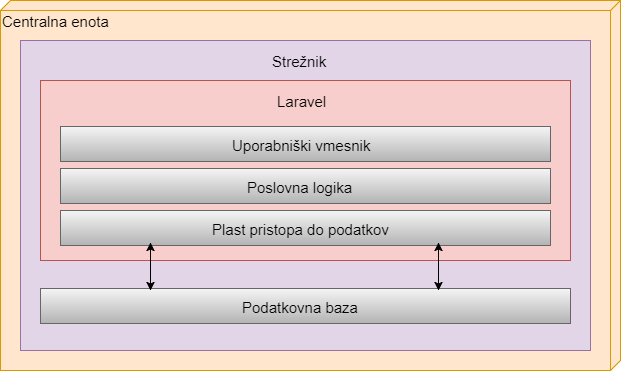
\includegraphics[width=1\linewidth]{Slike/CentralnaEnota.png}
\end{center}
\caption{Centralna enota.}\label{slika:CentralnaEnota}
\end{figure}

\subsection{Strežnik}
Strežnik bo služil zgolj za to, da bo centralna enota dostopna zunanjim uporabnikom (uporabniki in merilci) in za povezavo gradnikov, ki se bodo izvajali na njemu.


\subsection{Laravel framework}
Prva beta verzija Laravel 1 frameworka je bila napisana iz nič(od začetka??). in je bila izdana Junija 2011. Vsebovala je ORM(Eloquent) narejen po meri, closure-based routing, sistemski modul za extension in helpers za forme, validacijo, autentikacijo in več.

Zgodnji razvoj Laravel frameworka se je razvijal hitro. Laravel 2 in 3 sta bila izdana novembra 2011 in februarja 2012. Novosti v laravelu 2 in 3 so bili kontrolerji, unit testiranje, command line orodje, inversion of control(Ioc) container, Eloquent relacije in migracije.

Laravel 4 je bil ponovno napisan od nule(začetka???) in je bil izdan maja 2013 v novi strukturi, saj se je v tej točki composer(php's ubiquitous package manager) začel kazati za dober industrijski standard, kar je pokazalo velik potencijal za framework, napisan kot zbirka komponent, ki je bila povezana med seboj s strani kompozerja. Laravel je bil zato razvit kot zbirka komponent pod imenom Illuminate in od te točke naprej ni bil več na voljo kot download, ampak je uporabljal večino komponent od Symfony-ja(še en framework, ki dovoljuje uporabo komponent ostalim) in komponente Illuminate s pomočjo Composerja. Ker je laravel od tedaj naprej uporabljal veliko komponent symfony-ja, je prejemal 6 mesečne posodobitve, saj so sledili posodobitvam symfony-ja. Z izdajo Laravel 4 frameworka, so predstavili tudi vrste, mail komponente, facades, in database seeding.

Laravel 4.3 bi moral biti izdan novembra 2014, vendar so pri razvoju zaradi potrebe po velikih spremembah ugotovili, da ne bodo uspeli izdati nove verzije do omenjenega roka. Laravel 5 je bil zato izdan februarja 2015 z njim pa so prišle novosti kot so nova direktorna struktura, odstranitev helperjev za forme in html, introduction of the contract interfaces, a spate of new views, socialite for social media authentication, elixir for asset compilation, scheduler to simplify cron, dotenv for simplified enironmant management, form requests and a brand new repl(read evaluate print loop)


BOOK: LARAVEL UP AND RUNNING

\subsubsection{Zakaj Laravel}

Od vseh server-side programskih jezikov, je PHP eden od bolj popularnih. Nameščen je na veliki večini sistemov za web host in je tudi zelo enostaven za namestitev na osebne računalnike. PHP je dokaj enostaven, še posebej se znajdejo dobro začetniki, ki že imajo nekaj predhodnega znanja s htmljem, konceptom spremenljivk, inline conditions in include statementi. PHP ponuja tudi veliko pogosto uporabljenih funkcij, ki jih uporabljamo pri razvijanju spletnih strani. Seveda ima PHP zaradi svoje enostavnosti tudi nekaj drawbacks. Še posebej pri začetnikih, ki uporabljajo PHP velikokgrat pride do nepotrebne kompleksne kode, ki v večini primerov ni ločena po funkcionalnosti, saj nas nič ne prisili k temu. 

Velikokrat ko razvijamo aplikacije brez frameworka, imamo nekje spravljene že napise funkcije, katere pogosto uporabljamo za reševanje pogostih problemov kot so upravljanje s podatkovno bazo, autenticiranje uporabnokov... Problem pri tem je, da moramo sami skrbeti za vzdrževanje kode, kar lahko enostavno rešimo s frameworkom kot je laravel, saj nas med drugim prisili k ločevanju kode po funckionalnosti in skrbi za vzdrževanje že obstoječih funkcij.

BOOK: GETTING STARTED WITH LARAVEL

\subsubsection{Glavne funkcionalnosti}

\begin{itemize}
\item \textbf{Modularnost:} Laravel je bil zgrajen na več kot 20 različnih knjižnicah in je razdeljen v posamezne module. Ker je močno povezan z composer dependency managerjem, ga lahko zelo enostavno posodobimo.

\item \textbf{Preverljivost:}
Laravel je bil narejen z namenom enostavnega testiranja. Skupaj s frameworkom, je v paketu veliko metod, ki omogočajo obisk poti iz testov, pregled proizvedenega HTML-ja, zagotavljanje, da se metode izbranih razredov kličejo, impersioniranje autenticiranih uporabnikov...

\item \textbf{Usmerjanje:}
Laravel nam omogoča veliko fleksibilnosti ko definiramo poti naše aplikacije. Ročno lahko vežemo enostavno anonimno funkcijo na pot z HTTP metodo kot so GET, POST, PUT ali DELETE. Take funkcionalnosti izhajajo iz mikro-frameworkov kot so Sinatra (Ruby) in Silex (PHP). Poleg omenjenega je mogoče tudi priložiti filter različnim funkcijam, ki so izvedene na določenih poteh.

\item \textbf{Upravljanje konfiguracije:}
Aplikacije se zelo pogosto izvajajo v različnih okoljih, kar pomeni, da bo podatkovna baza ali pa e-pošni strežnik drugačen, različne bojo njihove nastavitve ali pa se bodo napake prikazovale na drugačen način, glede na to v katerem okolju se bo aplikacija izvajala. Laravel poenostavi omenjen problem, tako da, nam dovoljuje definiranje nastavitev za vsako okolje posebej in nato avtomatsko izbere pravilne nastavitve za izbrano okolje.

\item \textbf{Gradnja poizvedb in ORM:}
Skupaj z Laravelom dobimo metode za enostavno gradnjo poizvedb, ki nam omogočajo izvajanje poizvedb na bazi z uporabo PHP sintakse, kjer namesto pisanja zahtevnih SQL poizvedb, uporabimo enostavne metode. Poleg gradnje poizvedb z Laravelom dobimo metode za objektno relacijsko mapiranje (ORM) in Eloquent, ki so podobne tistim, ki jih najdemo v Ruby on Rails, ki skrbijo za povezavo modelov. Metode za gradnjo poizvedb in ORM so kompatibilne z različnimi podatkovnimi bazami, kot so PostgreSQL, SQLite, MySQL in SQL Server.

\item \textbf{Gradnja shem, migracije in sejanje:}
Kot veliko ostalih metod, so tudi te podobne tistim v Ruby in Rails. Dovoljujejo nam definiranje sheme podatkovne baze s PHP kodo in omogočajo sledenje spremembam s pomočjo migracij podatkovne bate. Migracije je enostaven način opisa spremembe sheme in kako jo razveljaviti. Sejanje nam dovoljuje enostaven vnos podatkov v podatkovno bazo, npr. po migraciji.

\item \textbf{Tempalte engine:}
Template engine je deloma podoben Razor predlogi jezika v ASP.NET MVC. V Laravelu se imenuje Blade in je enostaven način s katerim lahko naredimo hierarhično postavitev, s predefiniranimi deli kode, kamor lahko vstavimo dinamično vsebino.

\item \textbf{E-mail:}
Z razredom ki podpira pošiljanje elektronske pošte, lahko z uporabo popularne knjižnice SwiftMailer enostavno pošiljamo elektronsko pošto tudi z zahtevnimi vsebinami in priponkami.

\item \textbf{Autentikacija:}
Ker je dandanes autentikacija uporabnikov zelo pogosta funkcionalnost aplikacij, Laravel nudi orodja za registracijo, autentikacijo in celo prepošilljanje pozabljenih gesel uporabnikom.

\item \textbf{Redis:}
Redis je pomnilnik ki deluje na principu ključ-vrednost in je znan po svoji hitrosti. Če v Laravelu kreiramo instanco na katero se lahko Laravel poveže, jo lahko uporablja kot sejo in splošno namenski predpomnilnik s katerimi komunicira direktno.

\item \textbf{Vrste:}
Z laravelom lahko uporabljamo različne vrste, kot so Amazon SQS in IronMQ, ki nam omogočajo izvajanje zahtevnih opravil s časovnim zamikom. Zako lahko opravila kot so pošiljanje velikega števila elektronskih sporočil uporabnikom izvajamo v ozadju, namesto, da uporabniki čakajo, da se izvajanje konča.
\end{itemize}

\subsection{Podatkovna baza}



\begin{figure}[H]
\begin{center}
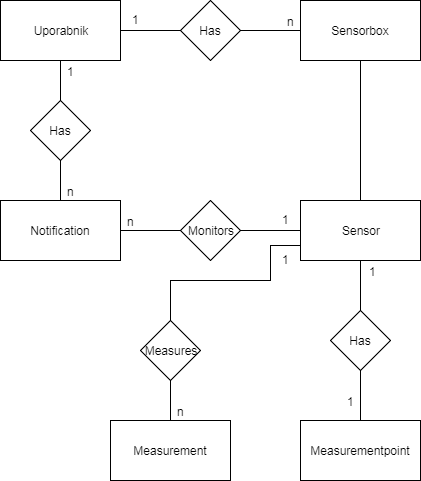
\includegraphics[width=1\linewidth]{Slike/ER.png}
\end{center}
\caption{ER diagram podatkovne baze.}\label{slika:ER}
\end{figure}


\begin{figure}[H]
\begin{center}
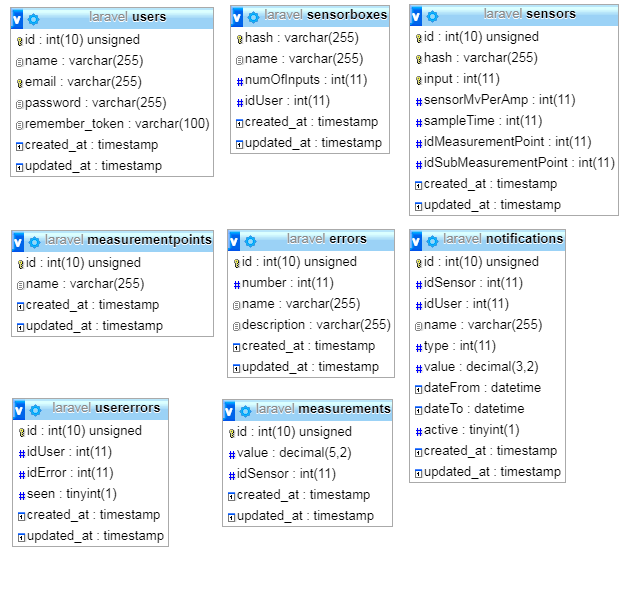
\includegraphics[width=1\linewidth]{Slike/DbTabele.png}
\end{center}
\caption{Tabele podatkovne baze.}\label{slika:DbTabele}
\end{figure}

\chapter{Izvedba}
\thispagestyle{fancy}
Pri izdelavi aplikacije smo uporabili različna orodja, ki so bila potrebna za izdelavo ali pa so nam olajšala delo.

\subsection{Composer}

https://getcomposer.org/doc/00-intro.md

Composer je orodje za upravljanje z odvisnostmi v PHP-ju. Omogoča nam da določimo knjižnjice, ki jih naš projekt potrebuje in nato avtomatsko poskrbi za njih (namestitve in posodobitve).
S pomočjo Composerja lahko kreiramo nov Laravel projekt. V našem primeru smo to storili z naslednjim ukazom:
\newline
\newline
\textbf{composer create-project --prefer-dist laravel/laravel ecc}
\newline
\newline
Po namestitvi lahko Laravel projekt zaženemo z naslednjim ukazom:
\newline
\newline
\textbf{php artisan serve}

\subsection{Git}

https://www.atlassian.com/git/tutorials/what-is-version-control



Version control systems are a category of software tools that help a software team manage changes to source code over time. Version control software keeps track of every modification to the code in a special kind of database. If a mistake is made, developers can turn back the clock and compare earlier versions of the code to help fix the mistake while minimizing disruption to all team members.

\subsection{ssh}
https://en.wikipedia.org/wiki/Secure\_Shell

Secure Shell (SSH) is a cryptographic network protocol for operating network services securely over an unsecured network.[1] The best known example application is for remote login to computer systems by users.

SSH provides a secure channel over an unsecured network in a client-server architecture, connecting an SSH client application with an SSH server.[2] Common applications include remote command-line login and remote command execution, but any network service can be secured with SSH. The protocol specification distinguishes between two major versions, referred to as SSH-1 and SSH-2.

\chapter{Testiranje}
\thispagestyle{fancy}


\section{Testiranje aplikacije:}
\thispagestyle{fancy}


\subsection{Registracija/prijava uporabnika v sistem:}
\subsection{Vnos novega merilca:}
\subsection{Urejanje in konfiguracija vnešenih merilcev:}
\subsection{Pregled porabe električne energije po merilnih mestih z možnostjo različnih filtrov:}
\subsection{Pregled porabe posameznega senzorja ("v živo"):}
\subsection{Dodajanje novih opozoril:}
\subsection{Urejanje že vnesenih opozoril:}
\subsection{Pregled napak in opozoril sistema:}
\subsection{Nadgradnja uporabnika v plačljivega uporabnika:}
\subsection{Pregled navodil za uporabo:}

\section{Testiranje merilca:}
\thispagestyle{fancy}


\subsection{Poizvedba nastavitev senzorjev:}
\subsection{Beleženje porabe:}
\subsection{Poročanje rezultatov meritev:}
\subsection{Okrevanje po napaki:}


\chapter{Zaključek}
\thispagestyle{fancy}






%\medskip
%\noindent Zgled citiranja:

%\medskip
%Minimiziranje pasovnosti matrik pomaga pri njihovem shranjevanju in pri računanju z njimi, npr.~pri Gaussovi eliminaciji. Bralec bo podrobnosti našel v~\cite{Chinn, George, Strang}.


%\begin{defi}
%Graf $G$ je {\em povezan}, če za vsaki dve točki $u,v\in V(G)$ obstaja vsaj ena $u$-$v$ pot v $G$.
%\end{defi}

%\begin{lema}
%Lema je pomožna trditev, ki služi za dokaz glavnega izreka.
%\end{lema}

%\begin{proof}
%Tu napišimo dokaz leme. Dokaz naj bo čim krajši, vendar razumljiv vsem študentom. Pazite na logično strukturo dokaza: Vsi koraki naj bodo utemeljeni.
%\end{proof}

%\begin{izr}
%Izrek je najpomemnejša trditev v poglavju. Izrekov naj bo čim manj, preostale trditve formuliramo kot leme ali kot trditve.
%\end{izr}

%\begin{proof}
%Tu napišemo dokaz izreka.
%\end{proof}

%\begin{posl}
%Posledica je ugotovitev, ki neposredno sledi iz glavnega izreka. Potrebuje le krajši dokaz (par vrstic). Če se ne da dokazati v par vrsticah, potem to ni več posledica, temveč lema ali trditev.
%\end{posl}

%\begin{prim}
%Z zgledom osvetlimo lemo ali glavni izrek. Zgled je lahko protiprimer k veljavnosti izreka, če mu izpustimo kakšno od hipotez.
%\end{prim}




%\begin{table}[h!]
%\caption{Algoritem PLOGBAND}
%\label{tabela:algoritem}
%\fbox{%
%\parbox{\linewidth}{%
%{\noindent \bf Algoritem PLOGBAND:}
%\vskip 5pt
%\indent Podatka: {\obeylines \indent \indent graf $G = G(V,E)$ na $n$ vozliščih in z $m$ povezavami,
% \indent \indent nenegativno celo število $L$.}
%\indent \indent $L \in \N$.}
%\begin{enumerate}

%\item Za $1 \le j \le L$ naj bodo $p_j$ približno enakomerno
%(geometrijsko) razporejena števila med $1 - 1/\log\log n$ in $1/\log n$.
%Tj., vsa razmerja $p_j/p_{j+1}$ naj bodo približno enaka. (Natančne
%formule so v~razdelku \ref{siroke}, kjer je opisana vložitev naključnih podmnožic.)

%\item Uredi vozlišča glede na naraščajoče vrednosti $h(v)$. Vozlišča z enakimi
%vrednostmi $h$ uredi poljubno.

%\item Vrni urejeni seznam vozlišč kot linearno ureditev.
%\end{enumerate}
%}}
%\end{table}

%\noindent Takole navedemo sliko ali tabelo:

%\medskip
%Vse, kar potrebujemo za konec dokaza, je povzeto v Tabeli~\ref{tabela:algoritem}.




%\medskip
%\noindent Podobno lahko označimo in navajamo razdelke, poglavja, izreke, ipd.



%
%\chapter{Naslov poglavja}
%\thispagestyle{fancy}

%Takole citiramo spletne vire:~\cite{splet1,splet2,splet3}.\\
%Takole citiramo članke, sprejete v objavo ali v tisku:~\cite{Novak,Novak2,Novak3,Novak4}.\\
%Takole citiramo članke, poslane v objavo:~\cite{Novak5,Novak6}.
%Za primer vhodih podatkov glej Sliko~\ref{slika:podatki}.



%%%%%%%%%%%%%%%%%%%%%%%%%%%%%%%% Literatura %%%%%%%%%%%%%%%%%%%%%%%%%%%%%%%%%

 \begin{thebibliography}{99}
\thispagestyle{fancy}

\bibitem{ComponrentsAndMethodsForCurrentMeasurement}
\spletniVirZAvtorjem
    {B.~Yarborough}
    {Components and Methods for Current Measurement}
    {http://www.vishay.com/docs/30304/currentmeasurement.pdf}
    {15}{6}{2017}

\bibitem{ACS712}
\spletniVirZAvtorjem
    {Allegro Microsystems}
    {Fully Integrated, Hall Effect-Based Linear Current Sensor with 2.1 kVRMS Voltage Isolation and a Low-Resistance Current Conductor}
    {https://www.sparkfun.com/datasheets/BreakoutBoards/0712.pdf}
    {16}{5}{2017}

\bibitem{MCP3008}
\spletniVirZAvtorjem
    {Adafruit industries}
    {2.7V 4-Channel/8-Channel 10-Bit A/D Converters with SPI Serial Interface}
    {https://cdn-shop.adafruit.com/datasheets/MCP3008.pdf}
    {25}{6}{2017}

\bibitem{SPI}
\spletniVirZAvtorjem
    {Motorola, Inc.}
    {SPI block guide V03.06}
    {https://web.archive.org/web/20150413003534/http://www.ee.nmt.edu/~teare/ee308l/datasheets/S12SPIV3.pdf}
    {25}{6}{2017}


\bibitem{PI}
\spletniVirZAvtorjem
    {Raspberry pi foundation}
    {Raspberry pi}
    {https://www.raspberrypi.org}
    {2}{7}{2017}

\bibitem{Arduino}
\spletniVirZAvtorjem
    {Arduino}
    {Arduino}
    {https://www.arduino.cc/}
    {12}{6}{2017}


\bibitem{RMS}
\spletniVirZAvtorjem
    {Electronics tutorials}
    {Electronics tutorials}
    {http://www.electronics-tutorials.ws/accircuits/rms-voltage.html}
    {12}{6}{2017}


\bibitem{SQROOT}
  \clanekVRevijiVecAvtorjev
    {J. F.~Kenney }{E.S.~Keeping}
    {Mathematics of Statistics, Pt. 1, 3rd ed.}
   { Princeton, NJ: Van Nostrand}
   {1962}{59-60}

\bibitem{LARAVELUPANDRUNNING}
  \clanekVRevijiVecAvtorjev
    {M.~ Stauffer}
    {Laravel: Up and Running}
   {O'Reilly Media, Inc.}
   {2016}{1. poglavje}


\bibitem{LARAVELSTARTED}
  \clanekVRevijiVecAvtorjev
    {R.~ Saunier}
    {Getting started with laravel 4}
   {Packt Publishing}
   {2014}{1. poglavje}


% Ena vrstica mora biti tu prazna zaradi pravilnih navedb na strani, kjer so reference citirane.
\end{thebibliography}
\newpage

%%%%%%%%%%%%%%%%%%%%%%%%%%%%%%%%%%%% Priloge %%%%%%%%%%%%%%%%%%%%%%%%%%%%%%%%%%%%%
\pagestyle{fancyplain}
\vspace*{\fill}
     \begin{center}
          \bf{\Huge{Priloge}}
     \end{center}
\vspace*{\fill}
\thispagestyle{fancy}

\appendix
\thispagestyle{empty}
\pagenumbering{gobble}

\addtocontents{toc}{\setcounter{tocdepth}{-1}}
\appendices{A Naslov prve priloge}
\chapter{Naslov prve priloge}
\thispagestyle{empty}
Tu dodamo prvo prilogo.

% pozor:
% ukaz
% \thispagestyle{empty}
% mora biti prisoten na vsaki strani priloge (da se ne prikaže glava dokumenta)

\appendices{B Naslov druge priloge}
\chapter{Naslov druge priloge}
\thispagestyle{empty}
Tu dodamo drugo prilogo.

% Pozor:
% ukaz
% \thispagestyle{empty}
% mora biti prisoten na vsaki strani priloge (da se ne prikaže glava dokumenta)

\addtocontents{toc}{\setcounter{tocdepth}{2}}
\end{document}